\documentclass[tikz,border=12pt]{standalone}
\usepackage{amsmath}
\usetikzlibrary{arrows.meta,calc}

\begin{document}
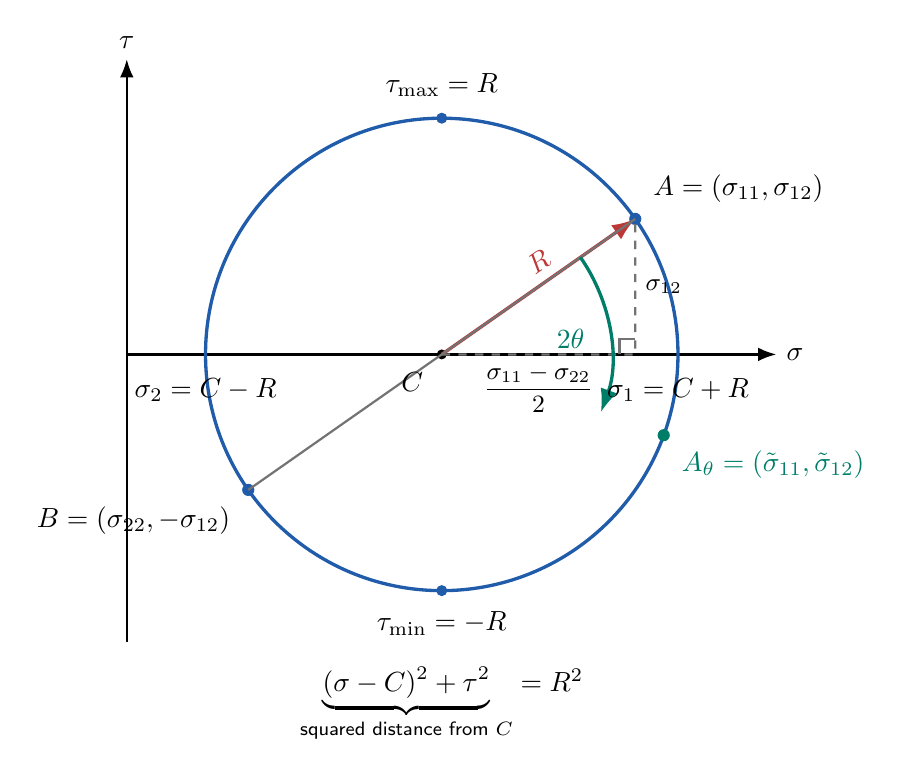
\begin{tikzpicture}[>=Latex,font=\sffamily,thick]
\definecolor{circlecolor}{RGB}{32,92,170}
\definecolor{radiuscolor}{RGB}{190,55,55}
\definecolor{anglecolor}{RGB}{0,125,105}
\definecolor{guidecolor}{RGB}{115,115,115}

% Schematic coordinates: center C=(4,0), radius=3, A is at 35 degrees.
\coordinate (C) at (4,0);
\coordinate (A) at ($(C)+(35:3)$);
\coordinate (B) at ($(C)+(215:3)$);
\coordinate (P) at ($(C)+(-20:3)$);
\coordinate (H) at (6.457,0);

% Stress axes.
\draw[->] (0,-3.65)--(0,3.75) node[above] {$\tau$};
\draw[->] (0,0)--(8.25,0) node[right] {$\sigma$};

% Mohr circle and characteristic points.
\draw[circlecolor,very thick] (C) circle (3);
\fill (C) circle (1.8pt);
\fill[circlecolor] (A) circle (2.2pt);
\fill[circlecolor] (B) circle (2.2pt);
\fill[anglecolor] (P) circle (2.2pt);
\fill[circlecolor] ($(C)+(90:3)$) circle (2pt);
\fill[circlecolor] ($(C)+(-90:3)$) circle (2pt);

% Radius and the right triangle behind the circle equation.
\draw[radiuscolor,very thick,->] (C)--(A)
  node[pos=0.56,above,sloped] {$R$};
\draw[dashed,guidecolor] (C)--(H)--(A);
\node[below,font=\small] at ($(C)!0.5!(H)$)
  {$\dfrac{\sigma_{11}-\sigma_{22}}{2}$};
\node[right,font=\small] at ($(H)!0.5!(A)$) {$\sigma_{12}$};
\draw[guidecolor] ($(H)+(-0.20,0)$)--($(H)+(-0.20,0.20)$)--($(H)+(0,0.20)$);

% Diameter endpoints representing two mutually perpendicular planes.
\node[anchor=south west,align=left] at ($(A)+(0.10,0.08)$)
  {$A=(\sigma_{11},\sigma_{12})$};
\node[anchor=north east,align=right] at ($(B)+(-0.10,-0.08)$)
  {$B=(\sigma_{22},-\sigma_{12})$};
\draw[guidecolor] (A)--(B);

% Rotation on the physical element by theta corresponds to 2 theta on the circle.
\draw[->,anglecolor,very thick]
  ($(C)+(35:2.15)$) arc[start angle=35,end angle=-20,radius=2.15];
\node[anglecolor] at ($(C)+(7:1.65)$) {$2\theta$};
\node[anchor=north west,anglecolor,align=left] at ($(P)+(0.10,-0.06)$)
  {$A_\theta=(\tilde\sigma_{11},\tilde\sigma_{12})$};

% Center, principal stresses, and maximum in-plane shear stress.
\node[below left=3pt] at (C) {$C$};
\node[below=5pt] at (1,0) {$\sigma_2=C-R$};
\node[below=5pt] at (7,0) {$\sigma_1=C+R$};
\node[above=4pt,align=center] at (4,3)
  {$\tau_{\max}=R$};
\node[below=4pt,align=center] at (4,-3)
  {$\tau_{\min}=-R$};

% Equation explained by the constant distance from C.
\node[align=center] at (4,-4.45)
  {$\underbrace{(\sigma-C)^2+\tau^2}_{\text{squared distance from }C}=R^2$};
\end{tikzpicture}
\end{document}
